\subsection{Accelerating the spectral element dynamics}\label{sec:homme-results}

We evaluate the impact of the threading changes described in Section \ref{sec:algorithm} using two different configuration of the HOMME dynamical core.  The {\em perfTest} configuration uses 26 vertical levels (plev=26), and 25 tracers (qsize=25) and is similar to how the default configuration of CAM-SE.  The {\em perfTestWACCM} uses 70 vertical levels (plev=70) and 135 tracers (qsize=135) and is comparable to the default configuration used by the Whole Atmosphere Community Climate Model (WACCM) \cite{waccm}.  HOMME uses a cubed-sphere computational grid, and horizontal resolution is indicated by the number of spectral elements on a side of a cube (ne). CAM-SE is typically run in production at ne=30 which corresponds to grid points approximately every 100 km.  High resolution simulations with grid points approximately every 25 km (ne=120) typically require very large core counts for an extended periods of time.   For example ASD simulation \cite{small2014} executed CAM-SE at 25 km resolution on 21,600 cores of Yellowstone in {\color{red} 20?? for ?4? months}.

%The performance of HOMME is strongly influenced by the number of spectral elements allocated to each hardware core.  The total number of spectral elements is calculated by the formula $nelem= 6 NE^2$, where {\em nelem} is the total number of elements.   For the 1/4 degree ASD simulation \cite{small2014} ne=120 (nelem=86,600) a total of 21,600 hardware cores were used resulting in the assignment of 4 elements per core.

 In order to evaluate that impact of our code optimizations we use several different horizontal resolution configurations (NE4, NE8, and NE30). The NE4 resolution has a total of 96 total spectral elements, while the NE8 and NE30 have 384, and 5400.  We use the NE4 and NE8 configurations to measure the impact of our modifications on either a single node or small number of nodes.  The NE30 configuration is to measure the impact of our modifications at much larger node counts.  


%Each spectral element consists of a [4x4] patch of grid points. 
% The Both configurations used [4x4] tensor product quadrature points within each element.  
%The experiments used for the performance studies were: perTestWACCM and perfTest with a baroclinic instability test case. These configurations were chosen as they represents the 'workhorse' for future experiments in the National Center for Atmospheric Research?s Community Climate System Model. Both experiments used NE=8 which represents a XX km horizontal resolution at the equator. The dynamics time-step for both cases was 480 seconds. For perTestWACCM there were 70 vertical levels with 135 tracers and for perfTest 25 vertical levels with 25 tracers. Both experiments used [4x4] tensor product quadrature points within each element. 

The execution time seconds/model day on Yellowstone and the computational cost for both the original ({\em orig})  and optimized ({\em opt}) code is provided for the NE4 configuration in Figure \ref{fig:homme-ys-ne4-cam}. In Figure \ref{fig:homme-ys-ne30-cam} a similar plot of execution time and computational cost is provided for the NE30 configuration.  Note that the number of nodes is on the x-axis on Figure \ref{fig:homme-ys-ne4-cam} and \ref{fig:homme-ys-ne30-cam}.  The left y-axis corresponds to the execution time in seconds per model day, while the right y-axis corresponds to the computational cost. The lines in Figures \ref{fig:homme-ys-ne4-cam} and \ref{fig:homme-ys-ne30-cam}, which are solid and dashed with diamond data points correspond to execution time while the dashed lines  correspond to computational cost.  Figures  \ref{fig:homme-ys-ne4-cam} and \ref{fig:homme-ys-ne30-cam} clearly illustrate that the {\em opt} code significantly reduces execution time versus the {\em orig} code.  For example for the NE4 resolution on a single node, the execution time is reduced from {\color{red} ??? to ?? a reduction of ??\%} a similar percentage reduction in execution time of {\color{red} ??\%} is seen on 57 nodes for the NE30 resolution.  It should be  noted that the choice of 57 nodes was not arbutratry, but rather intention so as to match the per hardware core problem size between the NE4 and NE30 resolutions.  Both  NE4 on a single node, and NE30 on 57 nodes of yellowstone assign 6 spectral elements per hardware core.  Both figures \ref{fig:homme-ys-ne4-cam} and \ref{fig:homme-ys-ne30-cam} also illustrate that NE4 and NE30 resolutions show similar scaling characteristics and speedup of the {\em opt} versus {\em orig} codes. It is for this reason that we believe a similar speedup will be apparently at a target production resolution of NE120 as well.   Figures \ref{fig:homme-ys-ne4-cam} and \ref{fig:homme-ys-ne30-cam} also illustrate that it is possible to scale HOMME to larger core counts.  In particular, while HOMME was previously limited to a single element per hardware core, It is now possible to obtain speedup for this configuration out to $1/4$ element per hardware core.
 
% KEEP
The plain dotted line and dotted line with diamond data points indicate the computational cost relative to the {\em orig} code are included in Figures \ref{fig:homme-ys-ne4-cam} and \ref{fig:homme-ys-ne30-cam} to illustrate the impact these optimizations may have on how HOMME is used in production.  While the {\em opt} version of HOMME will certainly reduce the cost of simulations on a fixed number of cores, it also introduces the possibility to use more hardware for a fixed computational cost.  For example in Figure \ref{fig:homme-ys-ne30-cam}, if we draw a horizontal line from the cost to run HOMME using 6 elements per hardware core from the original code (plain dotted line) to the optimized code (dotted line with diamonds) it is apparent that is is now possible to increase the amount of hardware used from 57 node to 675 nodes with only a 19\% increase in the computational cost.  The ability to efficiently utilize more hardware without increasing computational cost is an important advance for the {\em opt} code as it will allow HOMME effectively utilize systems with larger core counts.  Recall the ASD run which was run on 21,600 cores of Yellowstone, a per hardware core size of 4 elements per core.  Based it the the scaling results from Figure \ref{fig:homme-ys-ne30-cam} it is likely that future NE120 simulations which have 16 times the amount of parallelism as NE30, will be able to use 172,800 cores with a negligible increase in simulation cost.  

\begin{figure}
\begin{center}
\begin{minipage}{1.\textwidth}
   \begin{center}
   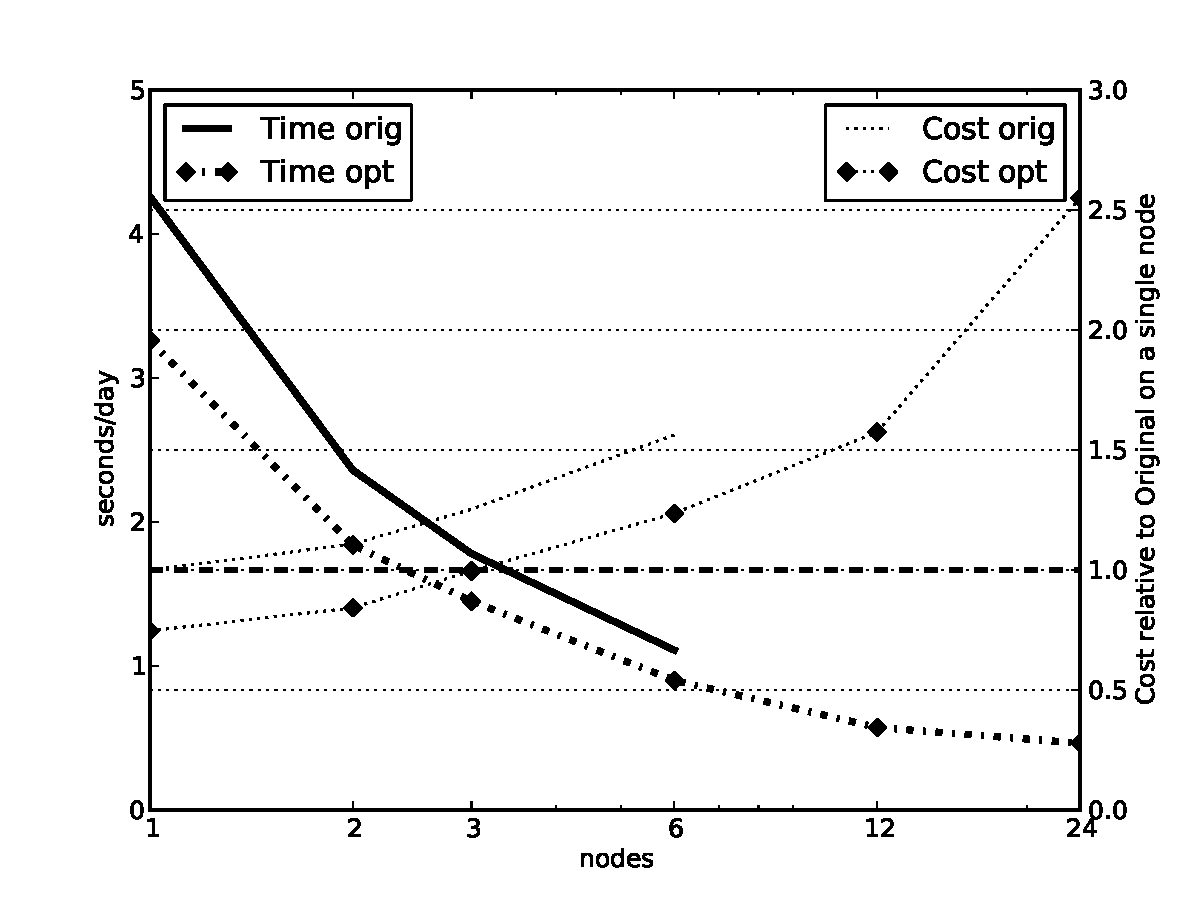
\includegraphics[width=1.\linewidth,height=.4\textheight]{figures/homme-ys-ne4-cam.pdf}
   \caption{NE=4 on 1-24 nodes.}
   \label{fig:homme-ys-ne4-cam}
   \end{center}
\end{minipage}
\begin{minipage}{1.\textwidth}
   \begin{center}
   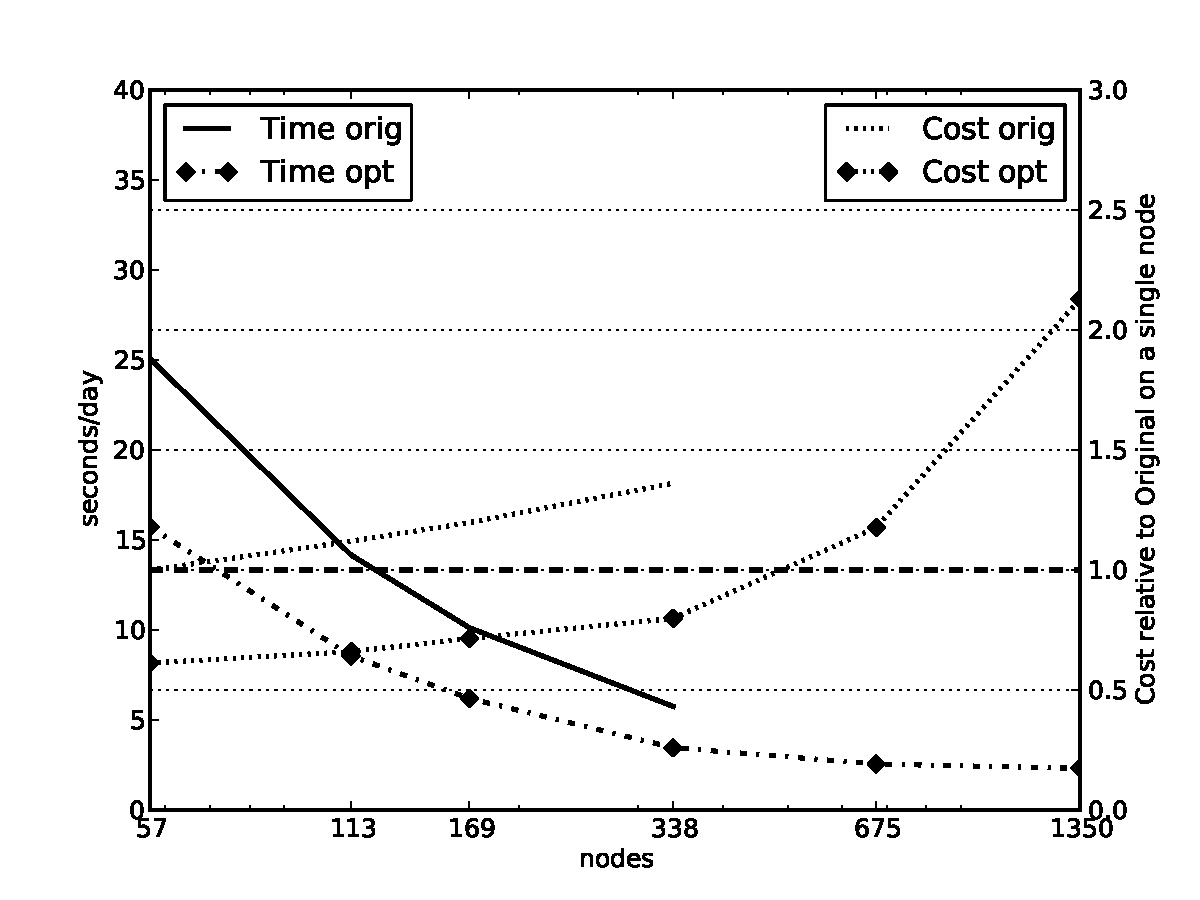
\includegraphics[width=1.\linewidth,height=.4\textheight]{figures/homme-ys-ne30-cam.pdf}
    \caption{NE=30 on 57-1350 nodes.}
    \label{fig:homme-ys-ne30-cam}
   \end{center}
\end{minipage}%
\caption{Strong scaling for HOMME in perfTest (PLEV=26, QSIZE=25) configuration on Yellowstone.  Note that each panel illustrates the execution time and computational cost of HOMME on core counts that range from 6 to 1/4 spectral element per core. }
\label{fig:homme-ys-ne4}
\end{center}
\end{figure}

%KEEP
The WACCM-like configurations has 70 vertical levels and 135 tractors (PLEV=70, QSIZE=125) as is similar to a standard configuration of the Whole Atmosphere Community Climate Model (WACCM).  Figures \ref{fig:homme-ys-ne4-waccm} and \ref{fig:homme-ys-ne30-waccm} illustrate both the execution time and computational cost of the {\em orig} and {\em opt} versions of the HOMME dynamical core.  The advantage of the {\em opt} versus {\em orig} code is even greater in the WACCM-like configuration.  For the 6 element per hardware core size, the {\em opt} reductions execution time by {\color{red} ??\%} for the NE4 resolution and {\color{red} ??\%} for the NE30 resolution. Due to the increased number of tracers and vertical levels, which represents additional threading parallelism, it is possible to scale to $1/8$ element per hardware core.  An evaluation of computational cost indicates that it is possible to run the {\em opt} version of HOMME in a WACCM-like configuration on {\color{red}????} nodes for {\color{red} ??\%} less then the {\em orig} code on 57 nodes.  

\begin{figure}
\centering
\begin{minipage}{1.\textwidth}
  \centering
  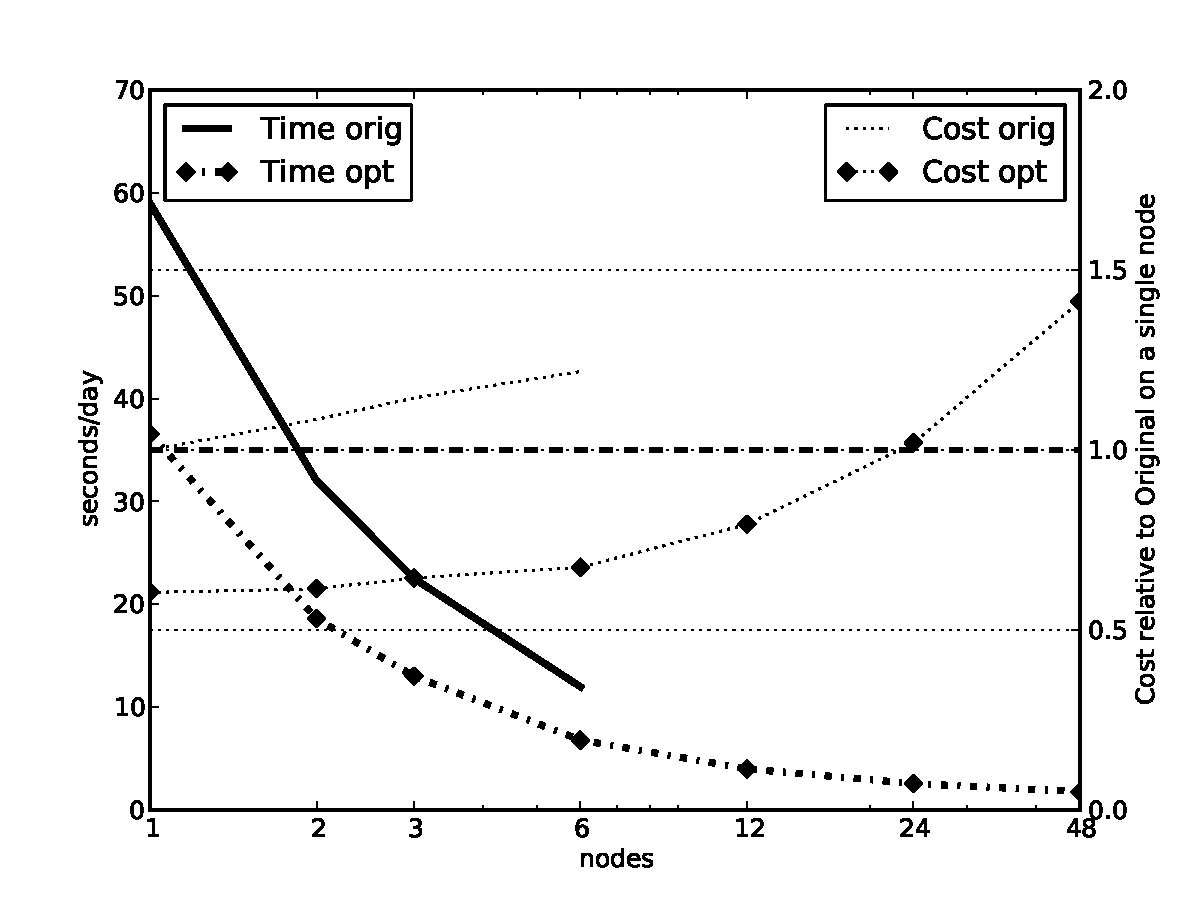
\includegraphics[width=1.\linewidth,height=.4\textheight]{figures/homme-ys-ne4-waccm.pdf}
 \caption{NE=4 on 1-48 nodes}
  \label{fig:homme-ys-ne4-waccm}
\end{minipage}
\begin{minipage}{1.\textwidth}
   \centering
   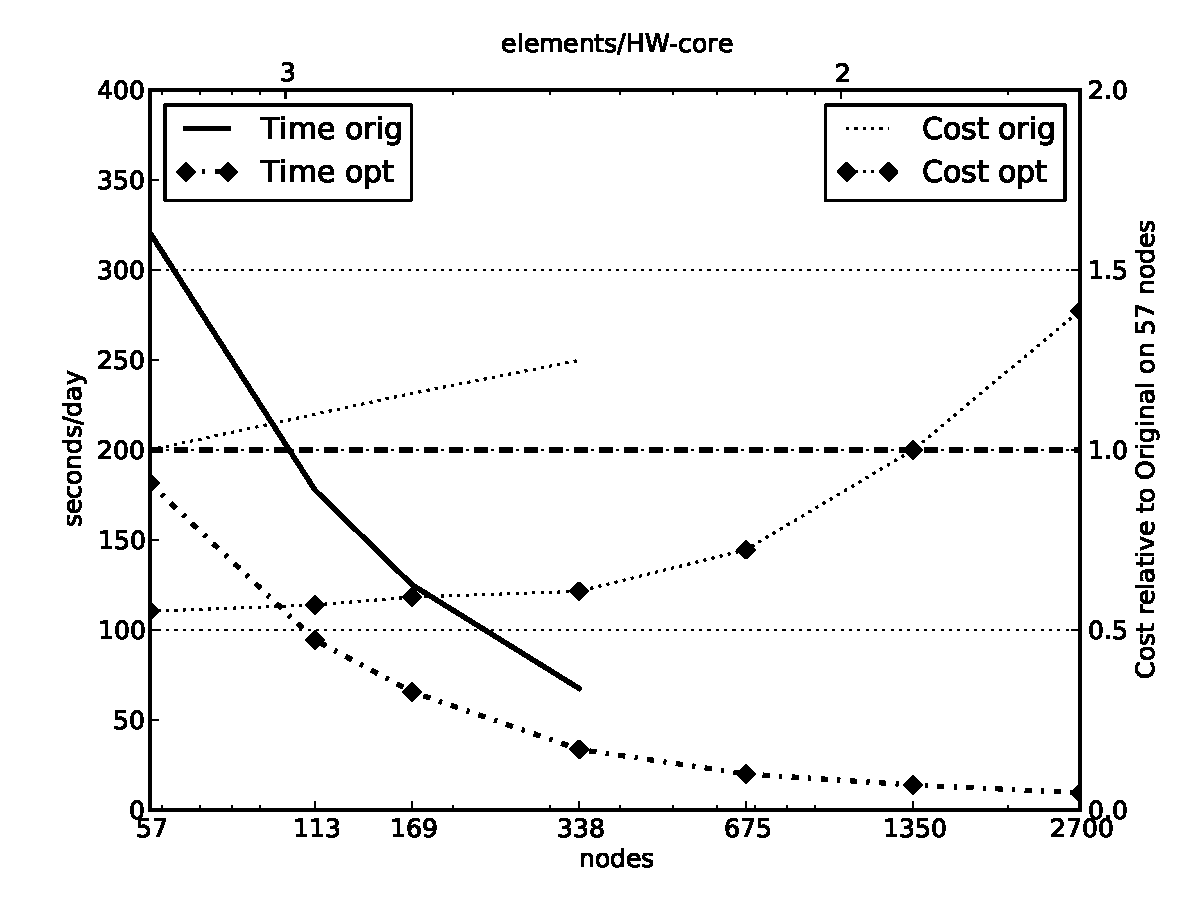
\includegraphics[width=1.\linewidth,height=.4\textheight]{figures/homme-ys-ne30-waccm.pdf}
   \caption{NE=30 on 57 to 2700 nodes}
   \label{fig:homme-ys-ne30-waccm}
\end{minipage}
\caption{Strong scaling for HOMME in perfTestWACCM  (PLEV=70, QSIZE=135) configuration on Yellowstone.  Note that each panel illustrates the execution time and computational cost of HOMME on core counts that range from 6 to 1/4 spectral element per core.}
\end{figure}

%KEEP
We examine the reason for the significant reduction in execution time for the {\em opt} versus {\em orig} code by looking at the way in which each code utilizes the underlying hardware.  In particular we use the extrae based folding technique described in Section \ref{sec:extra} and PAPI hardware counters \cite{papi} to examine the way in which each code interacts with the hardware.  We focus on the perfTestWACCM configuration at NE4 resolution on {\color{red} ??} nodes and examine the eulerian advection code in particular.  We sample a single MPI rank and plot the rates of L2 data cache misses, L3 total cache misses and 8-byte vector instructions, and plot these rates as a function of time for both the {\em orig} and {\em opt} codes.  Figure \ref{fig:perfTestWACCM-L2} illustrates the L2 data cache miss rates for both codes. The y-axis is in million of events/second, while the x-axis is normalized time.  The reduction in L2 cache miss rates for the {\em opt} versus {\em orig} code is significant, dropping from an average 70 to 17 Million events/second, a reduction of 76\%.  Figure \ref{fig:perfTestWACCM-L3} illustrates the L3 total cache miss rates for both codes.  For the L3 total cache miss rates for the optimizations reduced the total L3 cache miss rate from 11.1 to 6.5 Million events/second a reduction of 42\%.  The code modifications clearly significantly reduced the L2 and L3 cache miss rates.  Figure \ref{fig:perfTestWACCM-VEC} also illustrates that a significantly larger amount of the {\em opt} code is vectorized.  The amount of vectorized 8-byte floating-point operations increased from 253 Million events/sec to 1116 Million events/sec, and increase of 342\%

\begin{figure}
\centering
\begin{minipage}{1.\textwidth}
   \begin{center}
   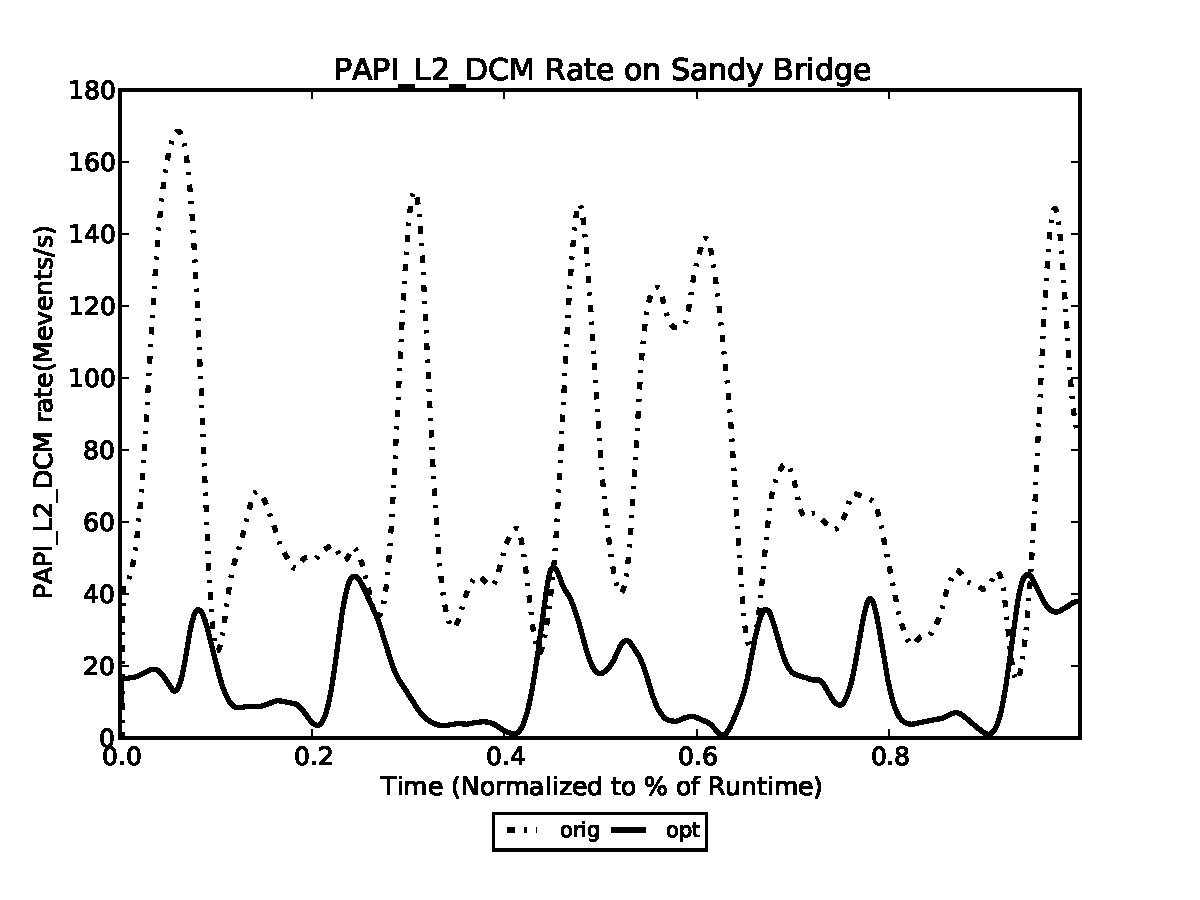
\includegraphics[width=1.\linewidth,height=.29\textheight]{figures/perfTestWACCM-PAPI_L2_DCM.pdf}
   \caption{L2 data cache miss rate}
   \label{fig:perfTestWACCM-L2}
   \end{center}
\end{minipage}
\begin{minipage}{1.\textwidth}
   \begin{center}
   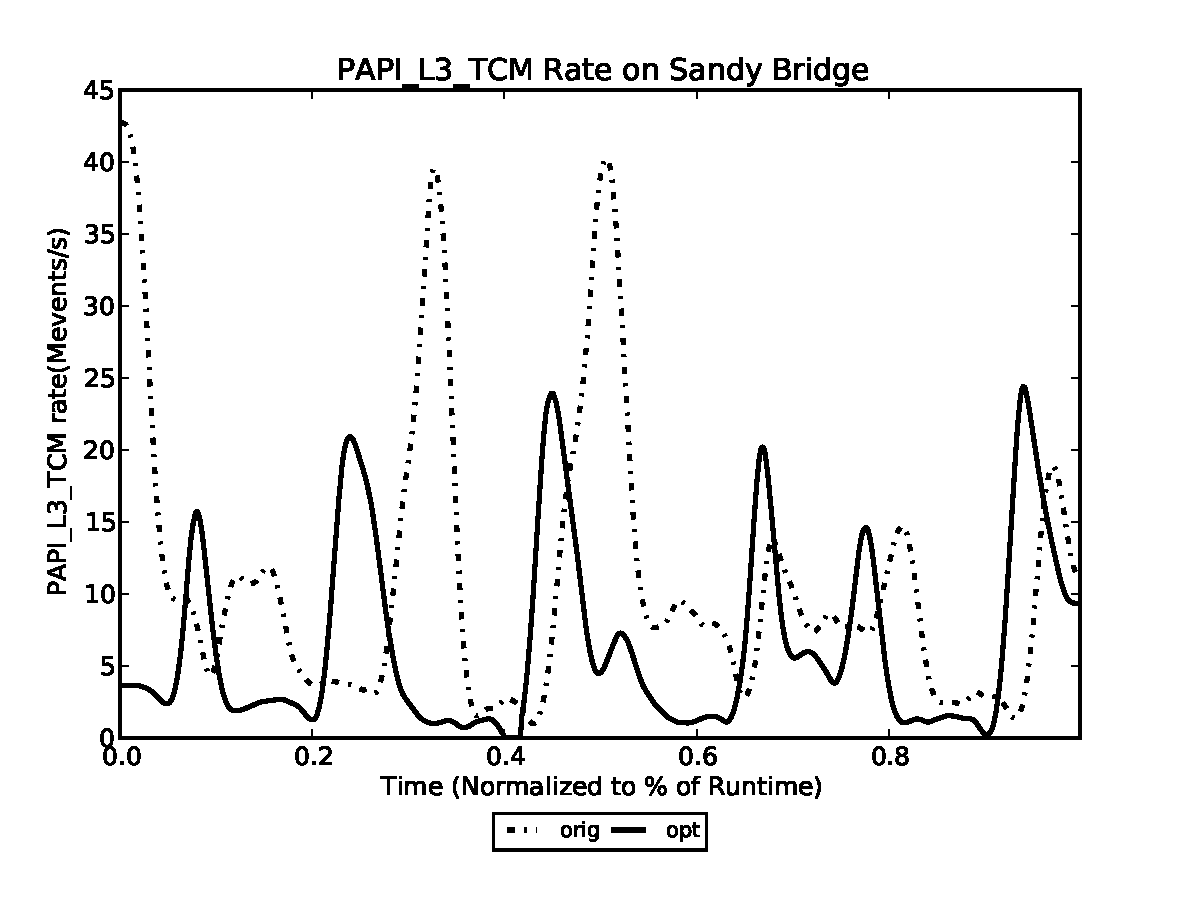
\includegraphics[width=1.\linewidth,height=.29\textheight]{figures/perfTestWACCM-PAPI_L3_TCM.pdf}
   \caption{L3 data cache miss rate}
   \label{fig:perfTestWACCM-L3}
   \end{center}
\end{minipage}
\begin{minipage}{1.\textwidth}
   \begin{center}
   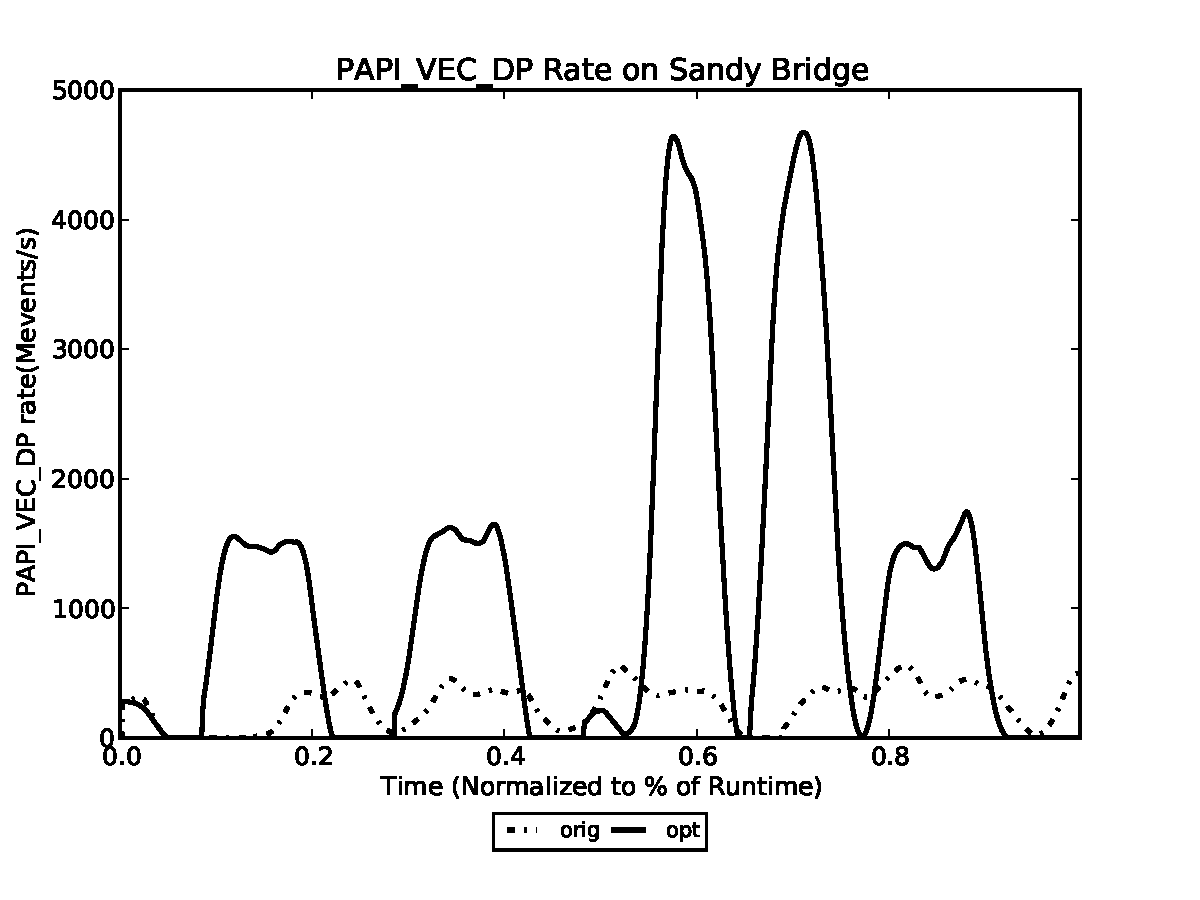
\includegraphics[width=1.\linewidth,height=.29\textheight]{figures/perfTestWACCM-PAPI_VEC_DP.pdf}
   \caption{8-byte real vector instruction rate.}
   \label{fig:perfTestWACCM-VEC}
   \end{center}
\end{minipage}
\end{figure}



Because of our IPCC-WACS project we have gained early access to single nodes of Knights Landing (KNL) hardware we are also able to provide timing results of the original and optimized SE dynamical core.  Using 68-core single socket system, we have been able to compare the performance of HOMME on both the CAM-like and WACCM-like configurations with a NE8 resolution.  In Figure \ref{fig:homme-knl-ne8-cam} the execution time for a number of different MPI and OpenMP configurations are provided for both the original {\em orig} and {\em opt} code bases.  Because the amount of parallelism in this problem is not to divisible by 68 we choose to idle 4 hardware cores, and configuration HOMME to use either 64, 128, 192, or 256 threads of execution.  Those configurations that use a 1, 2, 3, and 4, execution threads per hardware core are indicated by SMT{1}, SMT(2), SMT(3), and SMT(4) in Figure \ref{fig:homme-knl-ne8-cam}.  Recall from Section \ref{sec:somewhere} that the new version of HOMME  now supports threading over both the horizontal dimension as well as the vertical and tracer dimensions.  We define the particular parallel configuration of HOMME by the tuple 
$$
nRanks,  horz\_nthreads, max(vert\_nthreads,tracer\_nthreads)
$$
where $nRanks$ is the number of MPI ranks, $horz\_nthreads$ is the number of OpenMP threads in the horizontal dimension, $vert\_nthreads$ is the number of heads in the vertical dimension, and $tracer\_nthreads$ is the number of threads in the tracer dimension.  For example,  parallel configuration of {\em 8,16,2} corresponds to a configuration that uses 8 MPI ranks, 16 OpenMP threads over the horizontal and 2 over the vertical and tracer dimension, and has a total of 256 execution threads.   Despite the fact that we consider only those configurations that have a balanced number of spectral elements per MPI rank,  a total of 45 configurations are possible for the {\em opt} code base and 25 for the {\em orig} code base are possible.  In those cases where there are multiple configurations for a given number of MPI ranks we only plot the configurations with the lowest execution time.  A expected, Figure \ref{fig:homme-knl-ne8-cam} reveals a significant advantage for the {\em opt} code versus the {\em orig} code base.  The best execution time for the {\em opt} code for the CAM-like configuration at NE8 is {\color{red} ???} seconds a reduction of nearly {\color{red} ?63?\%} from the {\em orig} code.  For the {\em opt} code the best execution time is for the {\em 32,4,1} configuration with 128 execution threads while for the {\em orig} code it is for a {\em 128,1,1} configuration.  Both versions of code appear benefit from the use of multiple execution threads per hardware core, and prefer a larger number of MPI ranks and a modest number of OpenMP threads.  Interestingly, there appears to be a moderate penalty to using a total of 256 execution threads per node for the {\em opt} code.  It is also noteworthy that the {\em opt} version of the code appears to be more tolerance of moving parallelism from MPI ranks to OpenMP threads.  In particular, the performance impact of varying the number of on node MPI ranks from 8 to 128 is less then 10\%.  The ability the move from one type of parallelism to another with modest impact on performance may have a significant advantage when running HOMME on a system with multiple KNL nodes.  

The execution time for the WACCM-like configuration at NE8 on a single KNL node is provided in Figure \ref{fig:homme-knl-ne8-waccm}.  In the WACCM-like configuration, the minimum execution time for HOMME is {\color{red} 31.?} seconds is obtained on a {\em 64,2,2} configuration, and represents a nearly 75\% reduction in the execution. The WACCM-like configuration has a similar characteristics as the CAM-like configuration. In particular, best performance is achieved using 2 or more execution threads per hardware core.  Furthermore {\em opt} is also more tolerance of moving parallelism from MPI ranks to OpenMP threads.  

\begin{figure}
\centering
\begin{minipage}{1.\textwidth}
  \centering
  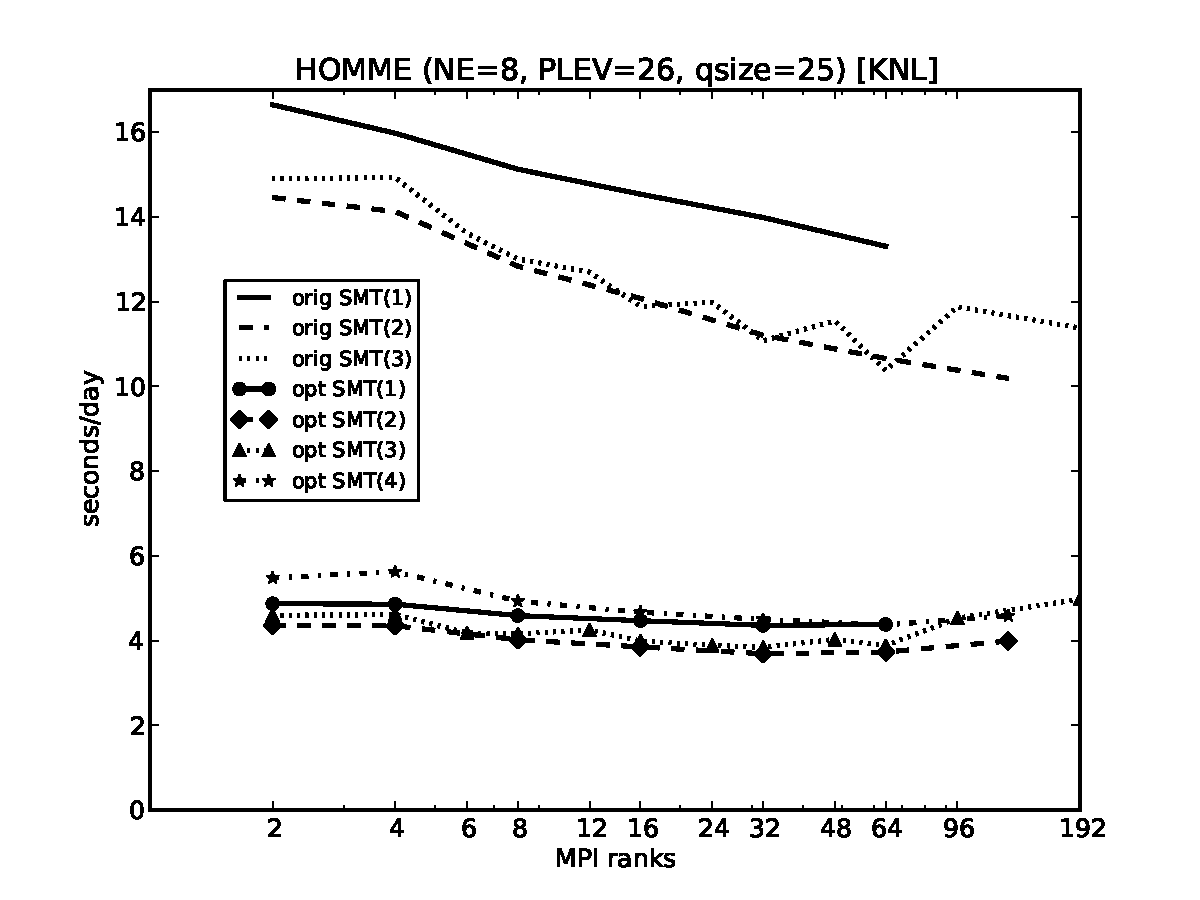
\includegraphics[width=1.\linewidth,height=.44\textheight]{figures/homme-knl-ne8-cam.pdf}
 \caption{A CAM-like configuration at NE8 (PLEV=26, QSIZE=25)}
  \label{fig:homme-knl-ne8-cam}
\end{minipage}
\begin{minipage}{1.\textwidth}
   \centering
   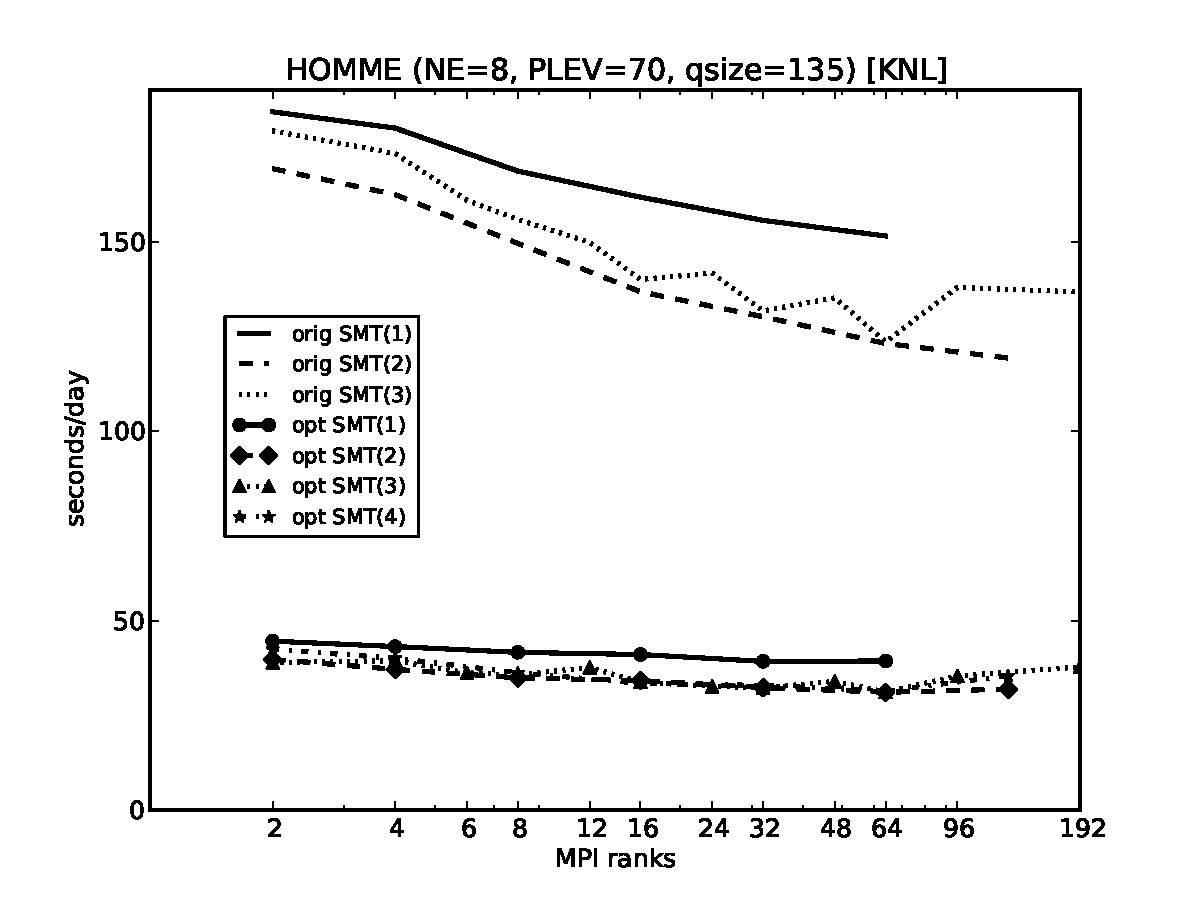
\includegraphics[width=1.\linewidth,height=.44\textheight]{figures/homme-knl-ne8-waccm.pdf}
   \caption{A WACCM-like configuration at NE8 (PLEV=70, QSIZE=135)}
   \label{fig:homme-knl-ne8-waccm}
\end{minipage}
\caption{Execution time for HOMME using 64 hardware cores of a KNL node.}
\end{figure}
